\documentclass[a4paper, 11pt]{article}
\usepackage{fullpage}

\usepackage[utf8]{inputenc}
\usepackage[swedish]{babel}

\usepackage{amsmath}
\usepackage{amsfonts}
\usepackage{amssymb}
\usepackage{graphicx}
\usepackage{float}
\usepackage{listings}
\usepackage{multirow}
\usepackage{fontenc}

\usepackage[hidelinks]{hyperref}

\usepackage{titlesec}
\setcounter{secnumdepth}{4}

\usepackage[backend=biber,style=numeric,sorting=none]{biblatex}
\addbibresource{cites.bib}

\usepackage{caption}
\captionsetup[figure]{name=Figur}


\begin{document}

\begin{titlepage}
\newcommand{\HRule}{\rule{\linewidth}{0.5mm}}
\begin{center}

\textsc{\Large }\\[2.5cm]
\textsc{\LARGE Uppsala Universitet}\\[1.5cm] 

\HRule \\[0.3cm]
{ \huge \textup {Historiekunskapsspel med semiautomatisk frågehämtning och ett balanseringssystem för frågor}}\\[0.3cm]
\HRule \\[1.5cm]


\Large \textsc{Författare:}\\[0.5cm]
\end{center}
\begin{minipage}{0.4\textwidth}
\begin{flushleft} \large
\large \textup{Alfred Yrelin}\\
\large \textup{Alfred.Yrelin.2125@student.uu.se}\\
\large \textup{\textup{Inst. för informationsteknolog}}\\
\large \textup{\textup{Uppsala Universitet}}
\end{flushleft}
\end{minipage}
~ \hfill
\begin{minipage}{0.4\textwidth}
\begin{flushright} \large
\large \textup{Josef Svensson}\\
\large \textup{Josef.Svensson.8440@student.uu.se}\\
\large \textup{\textup{Inst. för informationsteknologi}}\\
\large \textup{\textup{Uppsala Universitet}}
\end{flushright}
\end{minipage}

\center

\begin{minipage}{0.4\textwidth}
\large \textup{Philip Åkerfeldt}\\
\large \textup{Philip.Akerfeldt.4987@student.uu.se}\\
\large \textup{\textup{Inst. för informationsteknolog}}\\
\large \textup{\textup{Uppsala Universitet}}
\end{minipage}\\ [1.5cm]
~
{\Large \today}\\[2cm]
\vfill

\end{titlepage}

\newpage

\pagenumbering{gobble}
\begin{center}
\textbf{Förord}\\
\textit{Tack till}
\end{center}
\newpage
\tableofcontents
\pagebreak

\pagenumbering{arabic}



\section{Inledning}
Vem vill inte kunna avgöra diskussioner med sina vänner med argumentet "Jag är i alla fall bäst på ..."? 
Att tävla är både en rolig och en social aktivitet. Oavsett om målet är att vinna eller bara ha kul så bidrar spel ofta med någon form av tävlingskänsla. Att kunna få denna tävlingskänsla och samtidigt en källa för nöje så förmånligt i sin telefon är något som vi tror är något att eftersträva i mobila spel. Spel som exempelvis Quizkampen \cite{quiz} och Wordfeud \cite{wordfeud} besitter båda denna egenskap och det är därför vi tror att dessa spel har blivit så populära på marknaden \cite{appsalesrating}. Vi som utvecklare finner att Quizkampen och Wordfeud har lyckats väl med att designa spel som är enkla, roliga, estetiskt vackra samt effektiva i den meningen att man som spelare lätt kan orientera sig i applikationen. Vi eftersträvade att skapa ett spel som besitter samma egenskaper och som kan framkalla samma tävlingskänsla som i dessa spel. Ett spel som går ut på att ordna historiska händelser relativt till andra händelser. 

Applikationsutveckling för mobila enheter är ett spännande område som växer \cite{IDC}, under sista kvartalet av 2014 hade Android 81,5\% av marknaden och av de enheter som såldes hade 76,6\% Android som operativsystem. Enligt Digi-Capital-Found \cite{revenue} var även Android operativsystemet som gav högst intäkter för utvecklare som placerat sina applikation i någon form av applikationsmarknad, även om intäkter per nerladdning i iOS fortfarande var större. \\

VÅRT SPEL utvecklades till Android med en backend som drar nytta av Google App Engines skalbarhet för att ge applikationen möjlighet att växa i takt med användarantalet. För att vi inte skulle behöva söka och manuellt lägga in ett stort antal frågor utvecklades en semi-automatisk frågehämtare. Detta system bidrar till att VÅRT SPEL inte blir repetitivt och tråkigt för användarna. Frågehämtaren möjliggör att frågorna kan hämtas, skapas och läggas in utan att vi behöver tillägna mycket tid åt just dessa uppgifter. En annan sak som vi gjorde för att spelet skulle vara roligare för alla var att skapa ett balanseringssystem som gör att händelserna som ges till spelarna är anpassade efter spelarens kunskapsnivå.


\section{Bakgrund}
Denna sektion ger en översiktlig beskrivning av kategorier av spel var starkt relaterade till utveckling av vår applikation. Bland annat beskrivs kort några applikationer som var utvecklade på samma marknad. Det ges också en översiktlig beskrivning hur dessa applikationer och spel som, på ett eller annat sätt, använts vid utvecklingen av applikationen. 

\subsection{Kunskapsspel för mobiltelefoner}
Wordfeud och Quizkampen är två populära turbaserade multiplayerspel där Quizkampen har 45 miljoner användare globalt \cite{quiz} och Wordfeud har 20 miljoner användare \cite{wordfeud}. Dessa spel gör det möjligt att utmana vänner eller slumpmässiga personer på en match som spelas i omgångar. När en spelare spelar sin omgång får dess motståndare vänta på sin tur, vilket gör att en match kan pågå i flera dagar.

\subsubsection{Quizkampen}
Quizkampen \cite{aboutquiz} är ett frågesports-spel där spelarna svarar på frågor under 6 rundor med tre frågor i varje runda. Spelarna svarar på samma frågor varje runda.  Inför varje runda slumpas tre kategorier fram där endast en kategori väljs för den aktuella rundan. Valet av kategorier är något som spelarna turas om att göra varannan runda. Matchen avslutas när sista rundan är spelad och det är även då en vinnare koras beroende på vem som har flest poäng. 

\subsubsection{Wordfeud}
Wordfeud \cite{aboutwordfeud} är ett spel där en match utspelas mellan två personer. Varje spelare får en liten mängd bokstäver som är gömd för motspelaren. Spelet går sedan ut på att fläta samman ord på det givna spelbrädet med hjälp av bokstäverna. Målet är att få så många poäng som möjligt och detta kan man uppnå tack vare att varje bokstav är värd en viss poäng. På så sätt kan man genom att använda svårare bokstäver och skapa längre ord få mer poäng. 

\subsection{Sällskapsspel med fokus på kunskap}
Sällskapsspel har länge varit och är än idag ett populärt sätt att umgås på \cite{bradspelspop}. Sällskapsspelet \textit{När då då?} \cite{nardada} är ett spel har bygger på ett relativt enkelt koncept. Spelarna turas om att placera ut händelser på en tidslinje i förhållande till varandra och får poäng om dessa är korrekt utplacerade. Den spelaren som har flest poäng vid en slutet av matchen vinner. \\
Spelkonceptet är som sagt ett enkelt sådant men det är också kraftfullt i den meningen att det främjar vissa begär hos spelarna. Ett av begären är att man vill överkomma problem som ställs av antingen spelet själv eller motspelarna. Detta är en av faktorerna som gör den typen av spel så populära \cite{psykologi}.

\section{Projektbeskrivning}
Denna sektion lägger betoning på varför applikationen utvecklades. Vad som var våra mål med projektet, motivation för utvecklingen, vilka avgränsningar som gjordes, vilka krav vi ställde på applikationen, vilka tekniska problem vi var tvungna att överkomma samt vad som gjorde vårt spel unikt i förhållande till konkurrenterna.

\subsection{Syfte}
Det var projektets syfte att utveckla och distribuera en spelapplikation för mobila enheter som använder plattformen Android. Applikationen skulle ge flera användare möjlighet att interagera och spela med varandra samtidigt.

Spelet som utvecklades går ut på att två användare får tävla om vem som har bäst koll på när olika historiska händelser ägde rum. Varje spelare får ett antal händelser som hen sedan ska sortera i kronologisk ordning. Spelaren som sorterar flest händelser rätt vinner. Förutom rent nöje så kan spelet användas i utbildningssyfte. Detta i den meningen att det ger användaren en ypperlig möjlighet att förbättra sina kunskaper om historien.

\subsection{Mål}
Det fanns fyra stora delar i det här projektet som kan ses som projektets primära fokuspunkter. Målet vi hade för avsikt att uppnå är en mobilapplikation i form av ett spel. Spelet skulle köras på en server som har för uppgift att sköta all kommunikation mellan klienten och sig själv. En av de primära fokuspunkterna för spelet var att implementera en semi-automatisk informationshämtare som skulle fylla på spelets databas med nya frågor. Att informationshämtningen är semi-automatiskt betyder att ett steg i informationshämtningen kräver mänsklig interaktion. Interaktionen krävdes för att godkänna frågorna till databasen och detta är en uppgift som administratörerna (se avsnitt \ref{admins}) utför. 


\subsubsection{Mobilapplikation}
Vi strävade mot att utveckla en mobilapplikation till Android. Applikationen är det enda som användaren i slutändan ser och därför finn vi att kvaliteten av gränssnittet var extra viktigt i utvecklingen. 

Applikationen till Android skrevs i Java och gränssnittet skrevs med hjälp av XML \cite{xml}. 

\subsubsection{Server}
För att flera spelare skulle kunna interagera med varandra så behövdes det en server. En server möjliggjorde även att frågorna i spelet kunde uppdateras kontinuerligt under applikationens exekvering.

Servermjukvaran skrevs i programspråket Go \cite{golang} och kördes på Googles molntjänst App Engine.

\subsubsection{Automatisk informationshämtning}
För att spelet skulle bli så intressant som möjligt behövdes en stor bredd på frågorna som skulle lagras i spelets tillhörande databas. Ett sätt att skapa många frågor snabbt var att utveckla mjukvara som kunde hämta information och från denna informationen skapa nya frågor automatiskt. 

Målet med den automatiska informationshämtningen var att skapa ett delsystem som läste in delar av en hemsida, som följer en viss struktur, för att hitta nödvändig information. Systemet skulle sedan koppla samman årtalen och händelserna från hemsidan automatiskt. Systemet behövde också ett gränssnitt för att ge administratörerna ett snabbt sätt att korrekturläsa frågorna innan de godkändes och skickades vidare till spelet. För mer detaljerad information om mjukvarans design se avsnitt \ref{crawler}.

\subsection{Frågeställningar}

\subsubsection{Tekniska problem}
Det fanns vissa delar i det här systemet som blev mer avancerade att lösa än andra delar. En lista av följande utmaningar presenteras nedan.
\begin{itemize}
\item Eftersom applikationen på något sätt skulle hämta information och konstruera frågor på ett semi-automatiskt sätt var det ett måste att utveckla ett sådant system. En svårighet i detta var att se till att systemet blev tillräckligt smart för att lyckas läsa en informationskälla och ta ut den eftertraktade informationen på rätt sätt.
\item Det behövdes en relativt stor databas för att lagra både användare och frågor för spelet. Det här var något som vi inte hade arbetat med på en stor skala förut. Hur skulle man lagra informationen på ett sätt som var både effektivt lagringsmässigt samt snabbt och enkelt för servern att hämta?
\item Det krävdes nätverkskommunikation med säkerhet och användaridentifiering. App Engine som användes vid stora delar av utveckling hade användbara funktioner som uppfyllde vissa av våra krav men inte alla. Hur skulle vi lyckas tillgodose användarna med en säker applikation?
\item Spelet skulle anpassa svårighetsgraden automatiskt vilket innebar att någon form av balansering krävdes. Tanken var att frågorna skulle ha en svårighetsgrad som justerades automatiskt beroende på hur ofta de placerades rätt. Här var vi tvungna att ta hänsyn till hur resten av tidslinjen såg ut vid tillfället. Hur skulle detta utvecklas på ett tillräckligt effektivt och rättvist sätt för applikationen och användarna.
\item Det fanns ett behov att utveckla ett system för att rangordna spelare i någon slags topplista. Hur skulle detta ske och hur skulle rangordningen bestämmas utifrån spelets mekanik? 
\end{itemize}

\subsection{Relaterat arbete}
Det finns ett spel för iOS, \textit{Historiekampen} \cite{historiekampen} som också handlar om att lägga in händelser korrekt på en tidslinje. En nackdel som den befintliga iOS-versionen har är att användaren endast ser årtal på sin tidslinje, och inte vilka händelser som ligger där.

\subsubsection{Historiekampen}
Historiekampen var ett spel som konceptuellt sett liknade sällskapsspelet \textit{När då då?} väldigt mycket. En spelares tur gick till så att hen först fick en händelse som skulle placeras på spelarens tidslinje. När första frågan presenterades fanns det en årtalsreferens utlagd på tidslinjen som den första händelsen skulle placeras före eller efter. När nästa fråga presenterades fanns det två referenser (den första plus årtalet för frågan som precis placerades) och så vidare.\\ 
Historiekampen valde att använda konceptet med kombinations-poäng vilket implicerade att spelaren kunde få flera poäng under en runda om hen placerde ut flera händelser korrekt efter varandra. Spelaren var tvungen att placera minst \underline{en} händelse och kunde få maximalt tio händelser att placera ut. Om spelaren placerade första händelsen fel var avslutades rundan. Placerade spelaren händelsen rätt ställdes hen inför ett val med två alternativ: antingen avsluta sin runda och på så sätt låsa sina poäng, eller fortsätta att få händelser att placera ut i förhållande till de tidigare händelserna. Detta val gjorde spelaren efter varje rätt placerad händelse. Spelaren kunde med andra ord välja själv om den vågade fortsätta eller om den ville vara försiktig och behålla sina välförtjänta poäng. En duktig spelare kunde välja det senare alternativet och bygga upp sin kombo fram tills dess att den femte frågan var ställd. När den femte frågan var ställd fick hen en fråga om \underline{när} den femte händelsen ägde rum. Om spelarens svara var nära det rätta årtalet fick hen fortsätta rundan med sin uppbyggda kombo av poäng. Om årtalet var fel förlorade spelaren sina tidigare poäng men kunde fortsätta få händelser att placera ut i förhållande till de tidigare händelserna. Vid en perfekt runda kunde en spelare få totalt tio poäng.

\subsubsection{Balanseringsteori}
En viktig aspekt i det här projektet var att rangordna spelare i förhållande till varandra för att med hjälp av det skapa mer rättvisa matcher. Den här problematiken fanns det redan många som hade funderat på och de flesta större spel använder sig också av något system för detta. Två etablerade system är Elo och Glicko, varav Elo är det som har implementerats i det här projektet.

Elo är ett system som förutser hur stor del av en mängd spelade matcher som bör vinnas av vardera spelare, baserat på en den svårighetsnivå respektive spelare har. Det här systemet justerar, efter en match, poängen enligt beskrivningen ovan. Eftersom en lägre rankad spelare får fler poäng vid vinst mot en högre rättar systemet på sikt sig självt, vilket innebär att spelarna faktiskt får den nivå de förtjänar.

Elo-systemet fungerar enligt följande. Varje spelare får en initial Elo-poäng på 1000. Denna justeras sedan beroende på utfallet av en match i förhållande till det förväntade utfallet. Det förväntade utfallet beräknas:

$$E_A = \frac{1}{1+10^{(R_B-R_A)/400}}$$

Där $E_A$ är den förväntade andelen matcher som spelare A borde vinna. Är värdet till exempel 0.84 så innebär det att 84\% av matcherna borde vinnas av spelare A enligt nuvarande Elo-poäng. $R_B$ är spelare B:s nuvarande Elo-poäng och $R_A$ är spelare A:s nuvarande poäng.

När det förväntade utfallet har beräknats så justeras sedan spelarnas Elo-poäng enligt formeln:

$$R'_A = R_A + K(S_A-E_A)$$

Där $R'_A$ är spelare A:s nya Elo-poäng, $R_A$ är spelare A:s Elo-poäng innan matchen, $S_A$ är det faktiska utfallet av matchen och $E_A$ är det förväntade utfallet. K-värdet är en skalningsfaktor som justerar hur mycket poängen justeras vid varje vinst/förlust.

Ett räkneexempel med spelare A, 1300 poäng, och spelare B 1000 poäng, där A vinner:

$$0.849 = \frac{1}{1+10^{(1000-1300)/400}}$$
$$ R'_A = 1300 + 16(1-0.849) = 1302.416 $$
$$ R'_B = 1000 + 16(0-0.849) = 997.584 $$

I det implementerade balanseringssystemet används Elo-modellen för att beräkna spelarnas erfarenhetspoäng. Elo är ett system som utvecklades av Arpad Elo och började användas redan på 60-talet\cite{elo}. Systemet var först och främst utvecklat för att ranka schackspelare, men har sedan dess uppkomst även applicerats på många andra spel. Eftersom Elo-systemet är förhållandevis gammalt och möjligheten till datoriserade beräkningar blivit större sedan 60-talet, finns det mer avancerade system att använda sig av idag. Ett annat system som utvecklades i syfte att vara en förbättring av Elo-systemet är ett system kallat Glicko\cite{chessratings}. Skillnaden mellan Elo och Glicko är att Glicko också har ett värde för hur väl uppdaterad spelarens erfarenhetspoäng är. Det här innebär att spelaren har ett erfarenhetspoäng, säg 2000, samt ett trovärdighetspoäng, till exempel 100. Ju högre trovärdighetspoäng spelaren har, desto mindre exakt är erfarenhetspoängen. Erfarenhetspoängen har enligt systemet en +/- diff på dubbla trovärdighetspoängen. I nyss nämnda exempel innebär detta att spelaren har en erfarenhetspoäng på 1800-2200. Trovärdighetspoängen justeras bland annat baserat på hur länge sedan det var spelaren spelade förra gången, samt hur många matcher spelaren spelat totalt. Ju fler matcher totalt och ju närmare i tid förra matchen var, desto lägre trovärdighetspoäng har spelaren.

Både Elo och Glicko används idag och det verkar vara svårt att avgöra om Glicko verkligen är bättre än Elo\cite{stackchess}. Ett faktum som finns är i alla fall att Glicko kräver mer information för att kunna fungera. En faktor som Glicko behöver men inte Elo är en tidsvariabel som har reda på hur länge sedan det var spelaren spelade sin förra match\cite{glickoex}. Det här gör att mer data behöver lagras i databasen, vilket är negativt ur kapacitetsperspektiv.

\subsubsection{VÅR APPS spets}
VÅRT SPEL liknar Historiekampen och \textit{När då då?} rent konceptuellt. Uppgiften som spelarna skulle utföra i vår applikation och uppgifterna som skulle utföras i Historiekampen liknade varandra mycket. I både Historiekampen och VÅRT SPEL var det spelarens uppgift att placera ut händelser rätt på en tidslinje. Spelmekaniken var dock annorlunda i vår applikation då varje match och varje runda behandlades annorlunda. I \textbf{VÅRT SPEL} fick varje spelare ett paket med sex frågor varje runda. En av dessa sex frågor agerade som referenshändelse på tidlinjen. Frågorna presenterades för spelaren en i taget och det var sedan spelarens uppgift att placera dessa i rätt ordning. En spelare fick ett poäng per korrekt utplacerad händelse och kunde på så sätt få maximalt fem poäng från de korrekt placerade händelserna. Om en spelare lyckades få en perfekt runda, där alla händelser placerades rätt, fick hen ett extra poäng vilket resulterade i en total summa av sex poäng. Likt Historiekampen avslutades en runda när en spelare hade placerat en händelse fel. Det som skiljde vår applikation i denna aspekt var vid fallet då en spelare hade tjänat ihop poäng från tidigare händelser. I Historiekampen förlorade spelaren alla sina tidigare poäng om hen svarade fel medan i vår applikation fick spelaren behålla sina poäng. Oavsett om spelaren lyckades placera ut alla händelser rätt eller inte så gick turen, efter fem frågor, över till motståndaren. När fem rundor hade spelats vann den spelare som hade svarat rätt på flest frågor totalt.  

En viktig detalj som skiljde VÅRT SPEL från Historiekampen var faktumet att spelaren såg beskrivningen av händelserna som hen placerat tidigare istället för bara årtalen. Vid avslutad runda visades även de korrekta årtalen för händelserna så att spelaren visste vilken ordning som hade varit den korrekta. \textbf{VÅRT SPEL} handlade med andra ord mer om att relatera händelser till varandra (dog Palme efter andra världskriget?) istället för att veta vilket årtal det skedde.

Med den semi-automatiska frågehämtaren, som kunde anpassas för olika informationskällor, var det enkelt för administratörerna att hämta nya frågor. Databasen med frågor kunde på så sätt expandera snabbt vid behov. Detta var något som skiljde oss från Historiekampen där alla frågor matades in manuellt. \\
Applikationen balanserade även frågorna kontinuerligt efter varje match vilket bidrog till att alla spelare tilldelades frågor som passade deras aktuella kunskapsnivå. Balanseringen i spelet kunde även byggas ut och göras mer avancerad om användarna skulle ge kritik på hur frågorna rankades. Det fanns egentligen inga gränser för hur avancerad balansering kunde göras vilket var en stor fördel som skiljde oss från konkurrenterna.


\subsection{Motivation}
Det finns många mobilspel som handlar om att två personer möts och mäter sina färdigheter inom ett visst område. Exempel på sådana applikationer är Quizkampen och Wordfeud som båda toppar säljlistorna för Androidspel \cite{appsalesrating}. Dessa spel följer en ganska enkel struktur och den bygger på att två personer kan möta varandra, svara på frågor eller lägga ord korrekt. På detta sätt får spelarna poäng som sen avgör vinnaren mellan de tävlande. Enligt säljstatistiken \cite{appsalesrating} är detta koncept något som är attraktivt för många användare. Spelet, vars utveckling beskrivs i rapporten, kombinerar koncepten från Quizkampen och Wordfeud i den mening att spelare ska svara på frågor samt att lägga in saker på sin rätta plats. 

En liknande version av vårt spel har också visat sig vara populär i form av sällskapsspel (\textit{När-då-då?}) \cite{nardada}. Detta var en av anledningarna till att förhoppningarna var höga att även vår applikation skulle bli populär på marknaden. Det finns för tillfället ingen variant av det här spelkonceptet till Android vilket ger \textbf{VÅR APP} stora möjligheter att lyckas.

\subsection{Avgränsningar}
Någon applikation för Windows och iOS fanns som en eventuell fortsatt utveckling efter Android men kom till utvecklingsstadiet ty ett större fokus på en bra applikation till Android prioriterades. Spelet skulle troligtvis få ett par kategorier för frågorna, men vilka dessa skulle vara var då inte bestämt. 

I applikationen fanns det många funktioner som skulle vara roliga och användbara, men inför projektet hade vi några funktioner som ansågs vara viktiga att ha med. Den viktigaste funktionen var att kunna hitta och spela en match. En funktion för att hitta och hantera vänner man har i spelet och även kunna se statistik över matcherna man spelat mot en vän. Dessa funktioner behövde så klart även implementeras på servern.

\subsection{Krav}
Systemet skulle klara av många spelare samtidigt, dock bara två per match. Något speciell tak för antalet användare var inte bestämt men med tanke på den otroligt solida grunden för skalbarhet som projektet stod på kunde ett mål för önskat antal användare bestämmas. Eftersom App Engine användes för servern så skulle det inte bli några problem med den enkla förklaringen att det var en tjänst som automatiskt skalade med hänsyn på belastningen \cite{appenginescalability}. 

Informationssökaren skulle tillsammans med den administrativa kontrollen ge frågor som håller hög kvalitet. En hög kvalitet innebar frågor som var relevanta och som följde den strukturen som vi har tänkt oss. Frågorna skulle vara lätta att läsa, förstå och samtidigt befinna sig i det breda spektrumet av svårighetsgrader vi hade i spelet. Sökaren för frågorna skulle också vara så pass bra att den administrativa kontrollen gick fort och att så lite som möjligt behövdes korrigeras efter att frågorna hade samlats in. För att applikationen inte skulle kännas alldeles för repetitiv skulle det finnas många frågor som dessutom var av varierande kategori. Det skulle även finnas minst 1000 frågor i spelet.

Designen av applikationen var något som var väldigt viktigt för oss. Kravet i början var att ha en intuitiv, responsiv och snygg design. Eftersom applikationen gjordes för Android skulle den också följa dess designmönstret Material Design \cite{MaterialDesign}.



\section{Implementation}
Denna sektion beskriver hur de målsatta delarna implementerades i applikationen. Applikationens systemstruktur och dess innefattande delar  förklaras och illustreras. Det finns även en grundlig genomgång av hur applikationen ser ut samt hur den fungerar, både för användare och systemadministratörer.

\subsection{Metoder}
Ett antal olika verktyg användes för att möjliggöra detta projekt. För utvecklingen och simulering av Android-applikationen användes Android Studio \cite{androidstudio}. Detta var ett kraftfullt verktyg som exempelvis kunde, på ett smidigt sätt, simulera applikationen i olika valbara miljöer i form av layouts för olika mobiltelefoner.\\
Google App Engine användes lokalt för att simulera serverapplikationen. När tidsperioden för testning var över användes fortfarande App Engine men då i Googles moln istället för lokalt. App engine var ett värdefullt verktyg i vår utveckling med den enkla förklaringen att de tjänster som erbjöds när man utvecklade och körde sina applikationer via denna motor var otroligt värdefulla. Det var bland annat lätt att underhålla applikationen och skala upp när trafik och data krävde det \cite{googleappengine}. För att läsa mer om App Engine se \ref{Google App Engine}. \\
Den primära källan för information till frågorna var under utvecklingsfasen Wikipedia men denna ersattes mot andra informationskällor vid ett senare skede. Detta förekom innan produkten färdigställdes.\\ 
Valet att inte använda Wikipedia som informationskälla i den slutgiltiga versionen av applikationen berodde på dess tvivelaktiga roll som en pålitlig källa. Wikipedia trovärdighet hade länge diskuterats och det fanns många rapporter som hade undersökt dess trovärdighet. Att använda Wikipedia för att bekanta sig med ett ämne var fullt acceptabelt men borde lämpligtvis ha granskats kritiskt innan den användes som källa. Faktumet var att processen för att skapa och redigera artiklar på Wikipedia ansågs vara något osäker. Detta berodde mycket på att hemsidan följde strukturen \textit{editable-by-all} vilket innebar att vem som helst kunde ändra artiklar och på så sätt vinkla artikelns innehåll. Detta implicerade såklart inte att alla artiklar hade råkat ut för detta öde men det bidrog till en viss osäkerhet vid användandet av denna hemsida som källa vid vetenskapliga rapporter \cite{wikipediacred}.

\subsubsection{Google App Engine} \label{Google App Engine}
Google App Engine var en \textit{Platform as a service}, vilket var en servicemodell för molntjänster. Det byggde på att användaren skapade en programvara med hjälp av färdigbyggda bibliotek och verktyg som leverantören tillhandahöll. Programmet man byggde i App Engine kördes på Googles infrastruktur och var uppbyggt så att man kunde utöka antalet användare obegränsat. Flera stora företag använde sig av App Engine när deras produkter skulle lanseras där några av de större företagen var Coca Cola, Rovio och Best Buy \cite{googleappenginecustomers}. 

\subsection{Systemstruktur}

\begin{figure}[H]
	\begin{centering}
	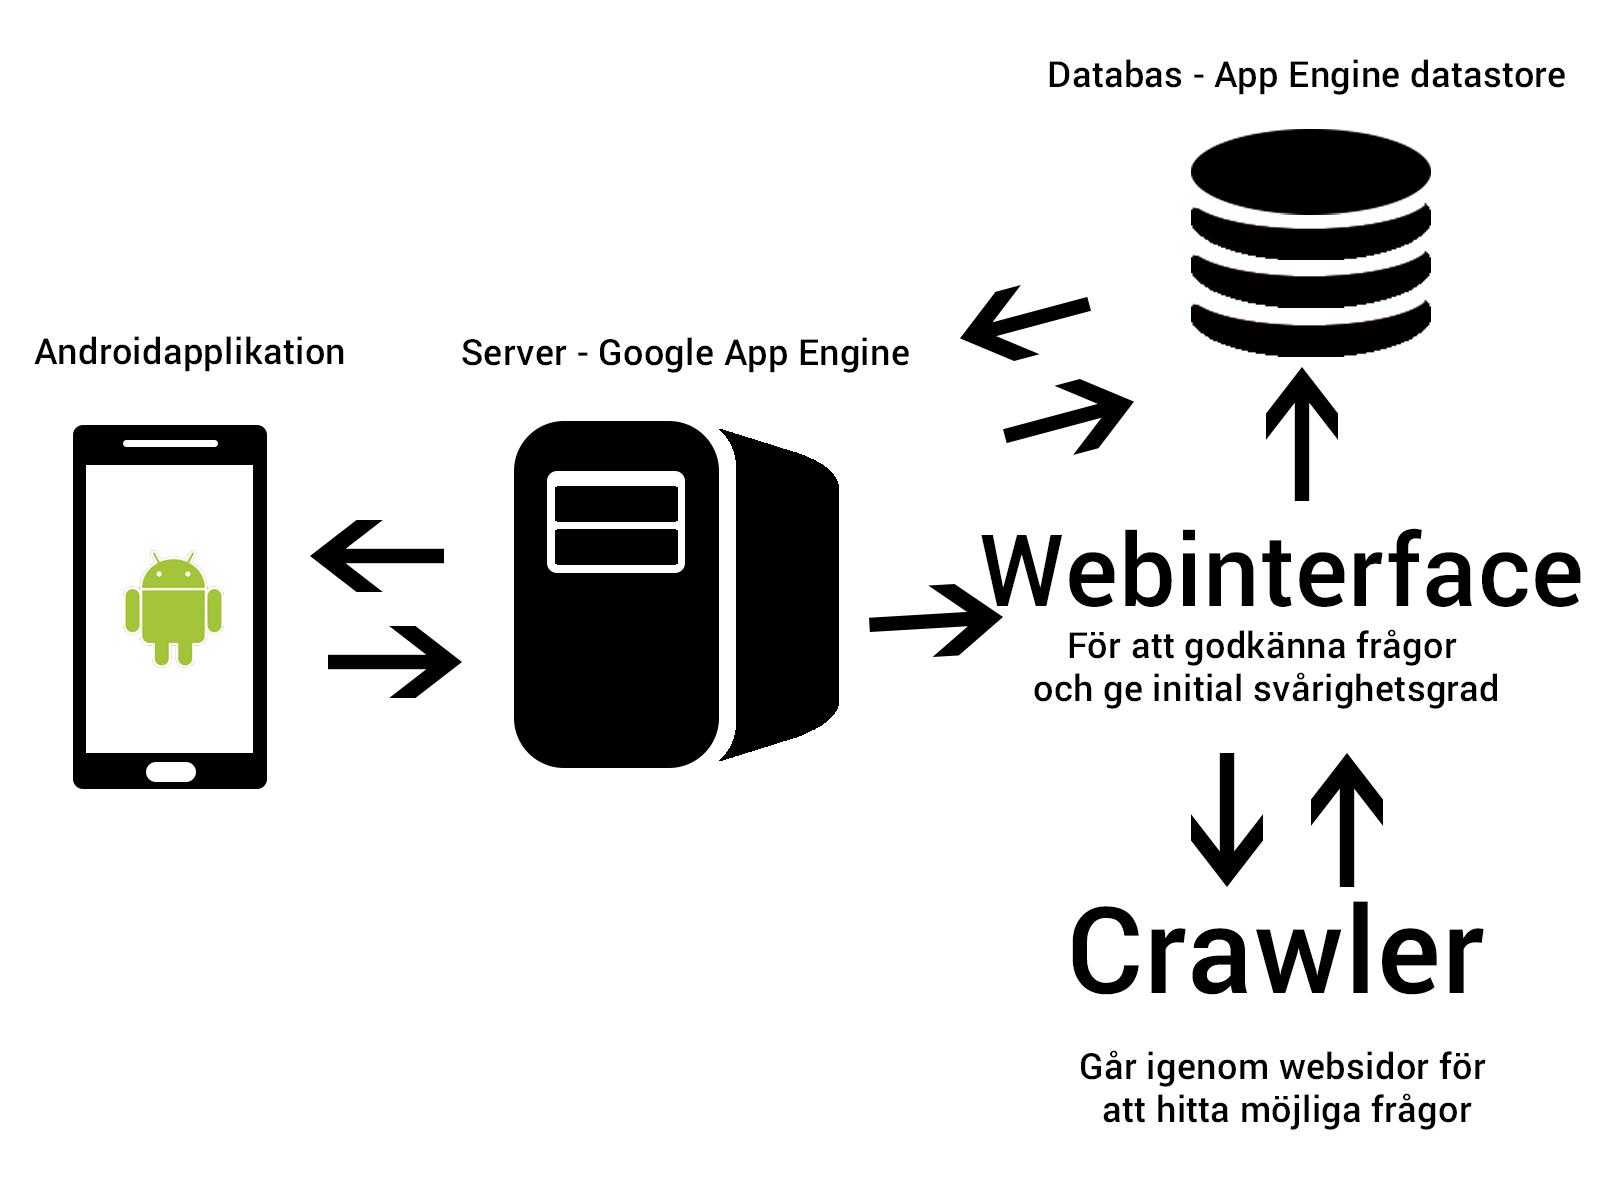
\includegraphics[width = \textwidth]{systemstruktur.jpg} 
	\end{centering}
	\caption{\textit{Illustration av systemstrukturen}}
\end{figure} 

\subsubsection{Androidapplikationen}
Androidapplikationen, klienten i systemet, var själva spelet som utvecklades. Det var den del av systemet som användaren interagerade med båda visuellt och funktionellt.

När det var den aktuella spelarens tur fick hen en chunk med sex frågor och dess svar (årtal) från systemets server. Svaren var gömda för användaren under rundans gång och användes endast av klienten för att rätta svaren från spelaren. När spelaren var färdig med sin runda och klienten hade rättat svaren så skickades dessa tillbaka till servern där de lagrades i matchens historik. 

\subsubsection{Server}
Klienten kommunicerade med en server som kördes i Google App Engine. Servern var utvecklad i programspråket Go (Golang) \cite{golang}. Anledningen till att vi valde att skriva servern i Go var för att det, enligt oss, var ett simpelt språk med en syntax som liknade andra språk som hade använts tidigare. Servern agerade även som en brygga mellan klienten och den databas som användes. När klienten krävde nya frågor till spelet kommunicerade servern med databasen. Databasen skickade frågor till servern som i sin tur skickade vidare till klienten. Utöver kommunikation till klienten och databasen användes även servern för att köra crawlern som var den semi-automatiska informationshämtaren. Servern hade också som uppgift att med jämna mellanrum köra fråge- och användarbalanseringssystemet som justerade svårighetsgraden på frågorna respektive spelarna i systemet. 

\subsubsection{Databas}
Databasen som servern kommunicerade med kördes, likt servern, i App engine med biblioteket \textit{datastore}. Datastore \cite{datastore} var Google App Engines egna bibliotek för hantering och lagring av data vilket innebar att systemet, utan vår assistans, hanterade all datalagring. Datastore hade flera egenskaper som bidrog till en enklare utveckling av resterande delar för projektet. Med tanke på att Datastore var ett bibliotek från App Engine så medföljde dess skalbarhet som skalade med beroende på behovet. Med Datastores inbyggda hjälpmedel för redundans kunde data lätt replikeras till flera datacenter om det skulle behövas. \\
Datastore hanterade datalagring med både SQL och NoSQL. För den som inte var bekant med NoSQL så var det en alternativ design för databaser som skiljde sig från SQL-databaser \cite{nosql}. NoSQL var designad på så sätt att det inte byggde på tabeller som i vanliga relationsdatabaser. Designen utvecklades för att möta kraven som då ställdes på datahantering. Marknaden som existerar då var vad som kunde kallas för en \textit{Big Data Reality} som kännetecknades av den enorma mängden data som var tvungen att hanteras i vardagen. NoSQL utvecklades för att bidra med en enklare design och lättare tillgänglighet. Det var mest datastrukturerna som skiljde NoSQL från vanliga relationsdatabaser. Detta ledde till att vissa operationer var lättare och mer effektiva att utföra i NoSQL medan andra var snabbare i vanliga relationsdatabaser \cite{nosqlfacts}. NoSQL användes alltmer av applikationer som var tvungna att hantera stora mängder data men också web-system som skulle exekveras i realtid \cite{nosqlcloud}. Egenskaperna som NoSQL hade passade för vår applikationen då ett tak för antalet användare inte var satt samt att vi önskade att exekvera i realtid.

Med Datastore behövde vi inte oroa sig över hur sökning och borttagning skulle ske i databasen. Detta kunde förklaras med att Datastore inte använde sig direkt av schemas som i en relationsdatabas, exempelvis SQL. Sökningen i databasen var också effektivt tack vare den solida sökmotorn som biblioteket tillhandahöll.

\subsubsection{Crawler} \label{crawler}
Inbyggt i servern fanns en form av crawler som hanterade den semi-automatisk informationshämtning av frågematerialet. Hela systemet hade som uppgift att givet en länk kunna läsa igenom sidan och dess undersidor för att hitta information som passade den mall för frågor som vi hade definierat. 

Sidor som visade sig vara enkla att läsa in var Wikipedias undersidor av typen listningssidor. Den här typen av sidor hade en punktlista med årtal samt en beskrivande mening av det årtalet inom den kategori som Wikipediasidan handlade om. Ett exempel var sidan som listar datorspelsår: Som återfinns vid denna  \textbf{\href{http://sv.wikipedia.org/wiki/Lista_\%C3\%B6ver_datorspels\%C3\%A5r}{länk.}} 
Denna struktur gjorde det enkelt att vid inläsning av en sida separera varje $<$li$>$-element där ett bindestreck eller kolon förekom och därefter spara varje kombination av årtal och händelse i ett temporärt cache.

\begin{figure}[H]
	\begin{centering}
	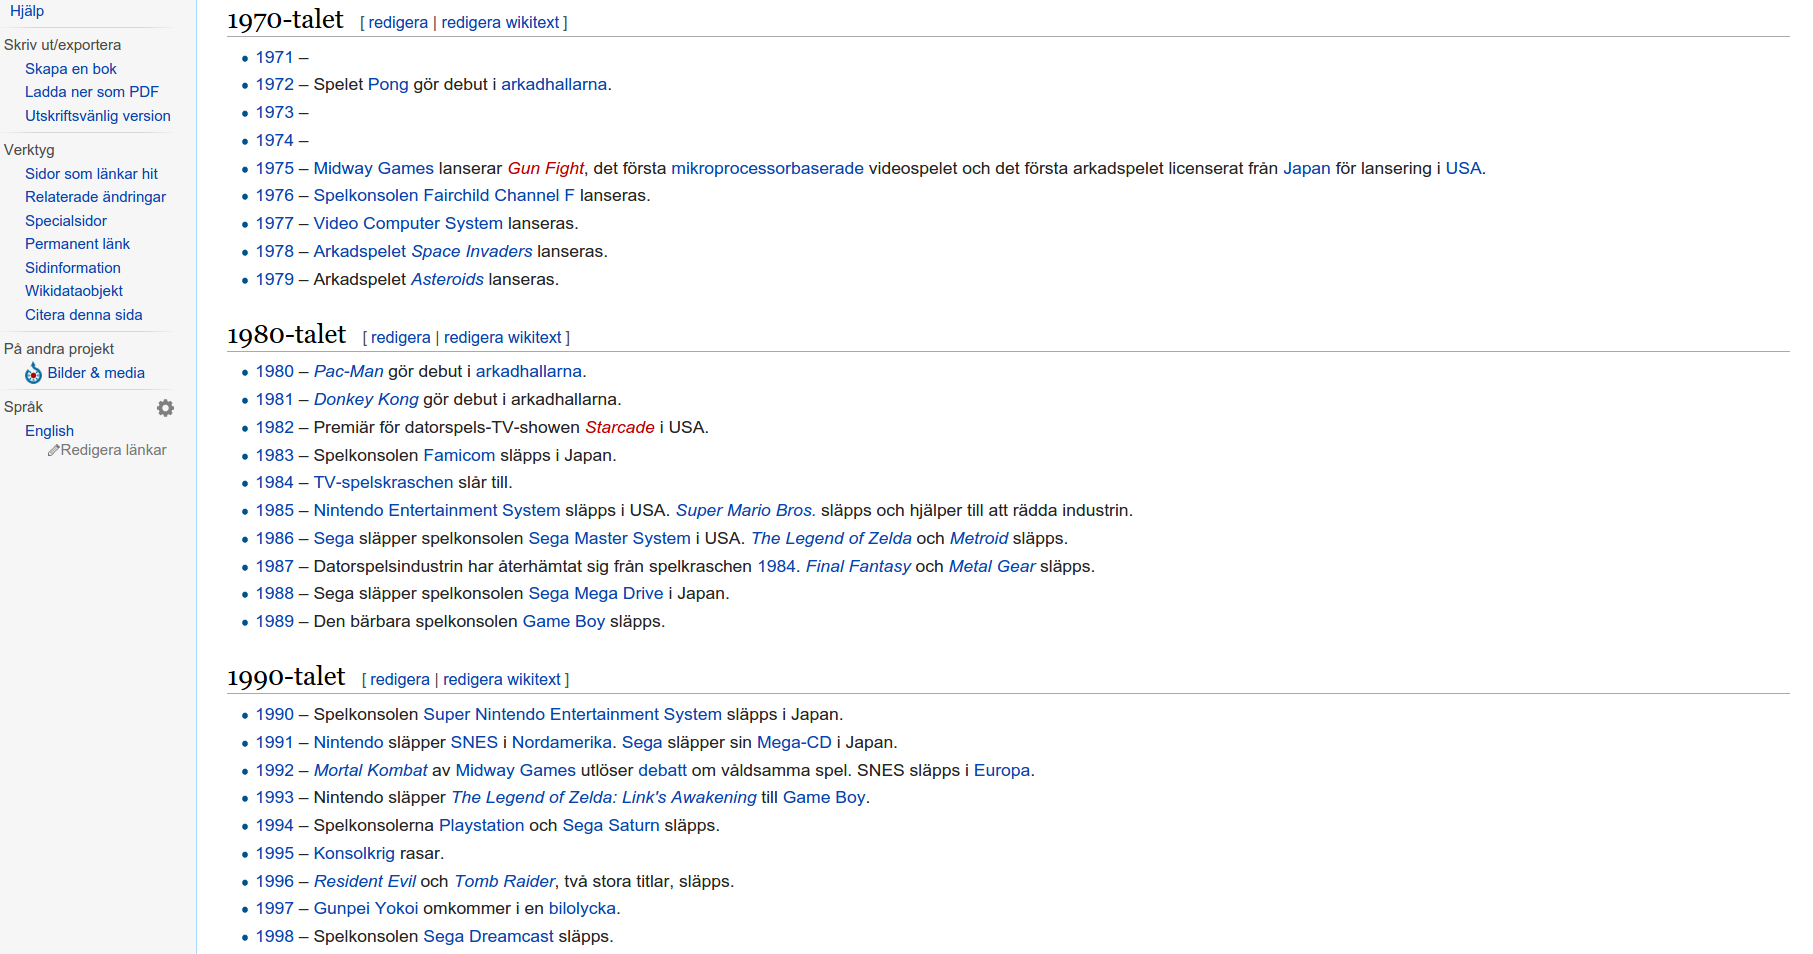
\includegraphics[width=\textwidth]{Listbild} 
	\end{centering}
	\caption{\textit{Ett exempel av listorna med årtal som Wikipedia tillhandahåller}}
\end{figure}

När alla  händelser hade lästs in i cachet presenterades de inlästa händelserna en i taget i ett webinterface. Webinterfacet visade ett årtal, en fråga samt fyra knappar. Knapparna angav svårighetsgraderna lätt, medel eller svår samt ett alternativ för att ta bort den aktuella frågan helt.

\begin{figure}[H]
	\begin{centering}
	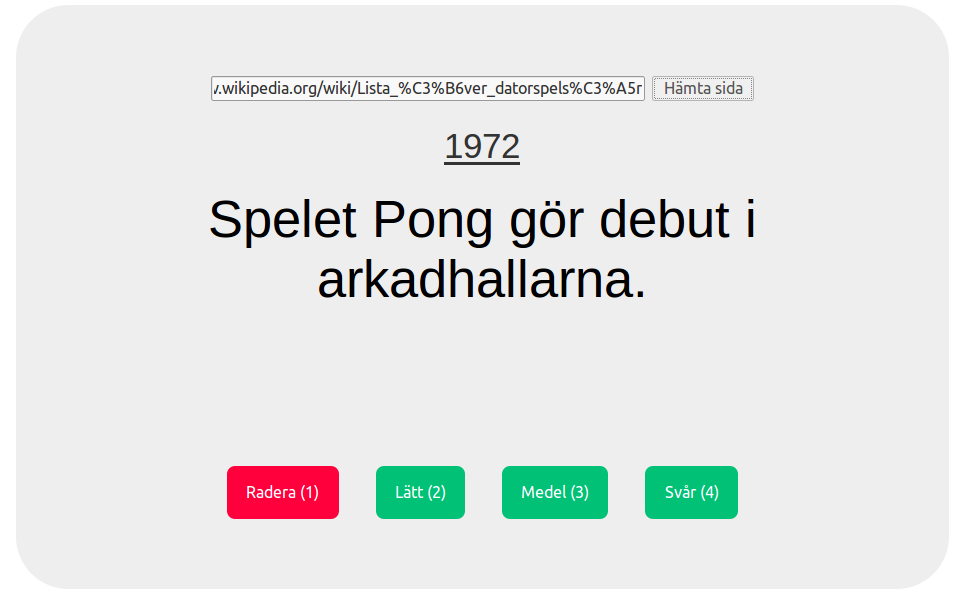
\includegraphics[width=\textwidth]{crawler} 
	\end{centering}
	\caption{\textit{Webinterface för crawlern}}
\end{figure}

De fyra knapparna var mappade till siffrorna 1-4 på tangentbordet för att det skulle gå snabbt att gå igenom frågorna. Texten kunde också redigeras om administratören ville justera grammatiska fel.

\subsubsection{Användare}
Det fanns två sorters användare som kunde interagera med systemet.\\
\newline
\textbf{Administratörer} \label{admins}
Administratörerna var vi som utvecklade applikationen och som arbetade med projektet. Vi var ansvariga för underhållet och utvecklingen av systemet. Vi hade den högsta typen av tillgång till systemet för att kunna utföra underhållet och utvecklingen. I underhållet innefattades det felsökning samt reparation av funna fel. Underhållet innefattade även uppföljning av rapporterade fel som skickats in av spelare. En vital uppgift som vi hade, förutom det allmänna underhållet och utvecklingen av systemet, var att godkänna informationen som hämtades av crawlern. Detta var för att se till att frågorna följde den struktur som vi fann lämplig för spelet.\\
\newline
\textbf{Spelare}\\
Spelarna var den typen av användare som hade en begränsad åtkomst till systemet. Spelarna kunde endast komma åt systemet genom klienten och kunde endast interagera med själva spelet. Detta innebar att en vanlig spelare inte kunde finna information om hur systemet fungerade. Detta var delvis en säkerhetsåtgärd som var till för att den vanliga användaren inte, av misstag, eller med flit skulle kunna komma åt systemets vitala delar och alternera dessa. Användaren kunde kommunicera med administratörerna genom att skicka felrapporter om spelet skulle bete sig konstigt eller om några buggar hade upptäckts.

\subsubsection{Balanseringssystemet} \label{balanseringssystemet}
Balanseringssystemet hade två mål, dels att justera svårighetsgraden på frågorna som fanns i databasen och dels till att justera spelarnas svårighetsgrad. 

Det fanns alltså två separata nivåsystem i applikationen. Varje fråga i databasen hade ett siffervärde för dess svårighetsgrad, ju högre siffra, desto svårare fråga. På liknande vis hade också varje användare en svårighetsgrad som lagrades som ett siffervärde i spelarens profil. Syftet med dessa poäng var att få spelet att sätta upp så rättvisa och roliga matcher som möjligt för spelarna. 

\paragraph{Balansering av frågorna}

Frågornas svårighetsgrad justerades beroende på hur spelarna i matchen svarade på frågan. En fråga som det ofta svarades fel på ökade i svårighetsnivå allt eftersom fler spelare svarade fel. Svårighetsgraden var helt bunden till frågan i sig och fanns alltså kvar mellan matcherna.

En frågas svårighetsgrad hade ingenting med någon form av poängräkning att göra. Svårighetsgraden på frågorna fanns till för att vid en matchstart kunna jämföras mot spelarnas svårighetsnivå. Med hjälp av detta kunde spelet avgöra om frågan skulle skickas till spelarna eller inte. Det handlade alltså helt och hållet om att spelet skulle presentera frågor som var lagom svåra för spelarna, så att spelet skulle bli lagom utmanande och maximalt roligt.

Om en spelare med låg nivå svarade rätt på en fråga så justerades frågans svårighetsgrad neråt. Ju högre nivå frågan hade, desto större blev nedjusteringen. En spelare med hög nivå påverkade inte frågorna lika mycket som en spelare med låg nivå. Det här berodde på att om en spelare med låg nivå svarade rätt på en svår fråga så var nivån på frågan förmodligen mycket mer felaktig än om en avancerad spelare svarat rätt på samma fråga. 

\paragraph{Balansering av spelarna}

Spelarnas svårighetsgrader justerades också efter avslutad match. Den här balanseringen gick i stora drag till så att den vinnande spelaren tog poäng av den förlorande spelaren. Om den vinnande spelaren redan låg på en högre nivå än den förlorande spelaren så tog hen väldigt lite poäng från förloraren. I det motsatta fallet tog istället den vinnande spelaren mycket poäng från den förlorande. Hur mycket poäng som faktiskt togs baserades på skillnaden i nivå mellan spelarna. 

Inspirationen till den här sortens balansering kom bland annat från Counter-strike: GO \cite{cs} som använder sig av balanseringssystemet Elo \cite{elo}. 

Balanseringen i \textbf{VÅRT SPEL} ansågs vara tillräckligt bra med Elo för att användningen av Glicko skulle uteslutas. Det var också förmodligen så att ett spel som schack eller Counter Strike behövde mer frekvent träning för att spelare skulle kunna behålla sin nivå än ett frågesportspel som \textbf{VÅRT SPEL}. Allmänkunskap och historiekunskap var någonting som lättare förbättras i vardagen, än till exempel schacktaktik. 

I \textbf{VÅRT SPEL} inträffade balanseringen efter en avslutad match. När hela matchen var avslutad fanns alla frågor från matchen samt respektive spelares svar i serverns cache. Efter att en vinnare hade utsetts anropades balanseringssystemet och både frågenivåerna och spelarnivåerna justerades utifrån matchens resultat.

\begin{verbatim}
downDiff = int((1.0-(userRatio*questionRatio))*10.0)
\end{verbatim}

Kodsnutten ovan är ett exempel på en justering som skedde om en spelare hade svarat rätt på den aktuella frågan. userRatio var ett värde mellan 0-1 på spelarens nivå (0 är nybörjare, 1 är avancerad). questionratio var ett värde mellan 0-1 på frågans nivå. downDiff var det värde som frågans nivå sänktes med (mellan 0-10). 

\subsection{Applikationens design}

\subsubsection{Genomgång av applikationen}
Gör en genomgång av hur aplikationen fungerar med en massa bilder som även har förklaringar till sig.


\section{Resultat}
Denna sektion beskriver ett antal utvärderingar som gjordes av applikationen. Utvärderingarna gjordes bland annat för att fastställa applikations användarvänlighet men också för att få nödvändig feedback på applikationens utseende och effektivitet.  

Här ska det skrivas MDI-utvärderingar
\begin{itemize}
\item Kognitiv walkthrough
\item Think aloud utvärdering
\item Heurisitc evaluation
\end{itemize}

\subsection{Utvärdering}
Planen var att en fungerande alfa eller betaversion av systemet skulle färdigställas en rimlig tid innan projektet avslutas. I den här versionen skulle användare ha möjlighet att ge feedback och att testa applikationen. Tack vare den feedback vi fick från användarna så skulle så många fel som möjligt justeras innan den färdiga versionen släpptes.

Gränssnittet och användandet av applikationen skulle också komma att utvärderas med hjälp av think aloud \cite{thinkaloud} och en heuristic evaluering \cite{heruistic}.

\section{Diskussion}
Denna sektion diskuteras det vad som hade kunnat göras bättre under utvecklingen. Exempel på detta kunde exempelvis vara om det fanns alternativa vägar eller verktyg som hade varit bättre, effektivare, enklare att använda. Det beskrivs även framtida utvecklingar i det visuella och applikationens prestanda och säkerhet.

\subsection{Alternativa vägar}

\subsection{Alternativa verktyg}

\section{Framtida utvecklingar för applikationen}



\newpage
\printbibliography[title={Referenser}]
\end{document}